\section{Schrijven}

\sectionframelogo{Kan een gestructureerd wetenschappelijk document schrijven, voorzien van referenties en conform de aangereikte template}

\begin{frame}{Structuur van een document}

    \centering
\begin{tikzpicture}[auto,thick,
deel/.style={ shape=rectangle,fill=HoGentAccent3,
  minimum width={width("Corpus/body")+24pt},draw}]

\node[deel] (1) [minimum height=24pt] {Samenvatting};
\node[deel] (2) [below=6pt of 1,minimum height=24pt] {Voorwoord};
\node[deel] (3) [below=6pt of 2,minimum height=56pt,fill=HoGentAccent1] {Corpus};
\node[deel] (4) [below=6pt of 3,minimum height=24pt] {Conclusies};

\end{tikzpicture}

\end{frame}

\begin{frame}{Samenvatting (Abstract)}

  \begin{itemize}
    \item max.~1 bladzijde
    \item Inhoud:
  \end{itemize}

\begin{description}
  \item [Context]:  Waarom is dit werk belangrijk?
  \item [Nood] :  Waarom moet dit onderzocht worden?
  \item [Taak]:  Wat ga je (ongeveer) doen?
  \item [Object]: Wat staat in dit document geschreven?
  \item [Resultaat]: Wat verwacht je van je onderzoek?
  \item [Conclusie]: Wat verwacht je van van de conclusies?
  \item [Perspectief]: Wat zegt de toekomst voor dit werk?
\end{description}

  \brightbox{Een samenvatting is \emph{geen} inleiding! Ook de (belangrijkste) conclusie(s) moeten hier in staan.}

\end{frame}

\begin{frame}{Samenvatting}
\framesubtitle{Voorbeeld abstract}

\begin{center}
  \only<1>{Context/nood}
  \only<2>{Taak}
  \only<3>{Object}
  \only<4>{Resultaat/Conclusie}
\end{center}

\scriptsize
\textbf{Energy-Efficient Resource Provisioning Algorithms for Optical Clouds}

\alert<1>{Rising energy costs and climate change have led to an increased concern for energy-efficiency (EE). As Information and Communication Technology (ICT) is responsible for about 4\% of total energy consumption worldwide, it is essential to devise policies aimed at reducing it.} \alert<2>{In this paper, we propose a routing and scheduling algorithm for a cloud architecture, which targets minimal total energy consumption by enabling switching off unused network and/or Information Technology (IT) resources, exploiting the cloud-specific anycast principle.} \alert<3>{A detailed energy model for the entire cloud infrastructure comprising wide area optical network and IT resources is provided. This model is used to make a single-step decision on which IT end points to use for a given request, including the routing of the network connection towards these end points. Our simulations quantitatively assess the EE algorithm’s potential energy savings, but also assess the influence this may have on traditional Quality of Service parameters such as service blocking. Furthermore, we compare the one-step scheduling with traditional scheduling and routing schemes, which calculate the resource provisioning in a two-step approach (selecting first the destination IT end point, and subsequently using unicast routing towards it).} \alert<4>{We show that depending on the offered infrastructure load, our proposed one step calculation considerably lowers the total energy consumption (reduction up to 50\%) compared to the traditional iterative scheduling and routing, especially in low to medium load scenarios, without any significant increase in the service blocking.}

\end{frame}

\begin{frame}[fragile]
  \frametitle{Refereren volgens de APA-stijl}
  Twee schrijfwijzen:
  
  \begin{enumerate}
    \item \textbf{Auteur (jaartal)} als de naam van de auteur een onderdeel is van de zin\\
    \LaTeX{}-commando: \verb|\textcite{key}|
    
    \framebox{\parbox{.8\textwidth}{\alert<1>{Ribas et al (2010)} schreven hierover een uitgebreid overzicht.}}
    
    \item zoniet \textbf{(Auteur, jaartal)}\\
    \LaTeX{}-commando: \verb|\parencite{key}|
    
    \framebox{\parbox{.8\textwidth}{Als je meer gedetailleerde informatie over Bib\LaTeX{} nodig hebt die niet in deze gids te vinden is, raadpleeg dan de handleiding \alert<2>{(Lehman, et al., 2016)}.}}
  \end{enumerate}

\end{frame}

\begin{frame}
  \frametitle{Refereren volgens de APA-stijl}
  
  \framesubtitle{Aandachtspunten}

  \begin{enumerate}
    \item Zijn de jaartallen van publicatie ingevuld?
    \item Zijn de auteursnamen correct? (i.h.b. organisatie)
    \item Staan de haakjes correct?
    \item Is de nodige info over de bron ingevoegd in de referentielijst?
    \begin{itemize}
      \item bv. URLs en datum van raadplegen
    \end{itemize}
  \end{enumerate}

\end{frame}


\begin{frame}[fragile]
\frametitle{Afbeeldingen invoegen}

\begin{columns}[c]
  \column{.65\textwidth}
  \begin{semiverbatim}
    \alert<1>{\\begin\{figure\}}
    \alert<2>{\\includegraphics[width=\\textwidth]
      \{img/knuth\}}
    \alert<3>{\\caption[Donald Knuth]\{Donald
      Knuth, auteur van \{\\TeX\}\}}
    \alert<4>{\\label\{fig:don\}}
    \alert<1>{\\end\{figure\}}
  \end{semiverbatim}
  
  \column{.35\textwidth}
  \begin{figure}
    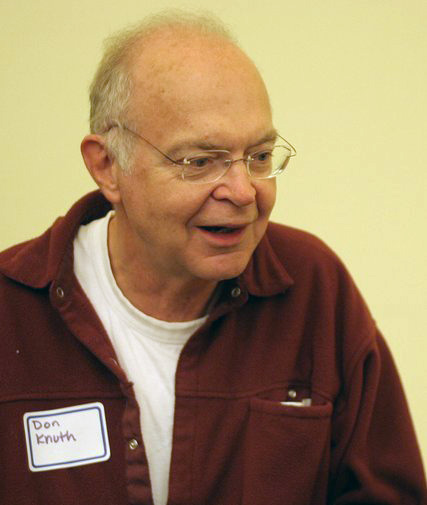
\includegraphics[width=\textwidth]{img/knuth}
    \caption[Donald Knuth]{Donald Knuth, auteur van {\TeX}}
    \label{fig:don}
  \end{figure}
  
\end{columns}

\end{frame}

\begin{frame}[fragile]
  \frametitle{Afbeeldingen invoegen}
  \framesubtitle{Aandachtspunten}
  
  \begin{itemize}
    \item Elke afbeelding heeft een bijschrift
    \item Overgenomen afbeelding? Bronvermelding nodig!
    \item Bijschrift geeft voldoende info om afbeelding te begrijpen
    \item In de tekst verwijzen naar de afbeelding met ``Zie Figuur NR''\\
    \LaTeX{}-code: \verb|Zie Figuur~\ref{fig:don}|
    \item GEEN logo's
  \end{itemize}

  \brightbox{Laat \LaTeX{} de positie van de afbeeldingen bepalen voor een optimale bladspiegel.}
\end{frame}

\begin{frame}{Tot slot}

\brightbox{Studenten die vast zitten met \LaTeX{} mag je doorverwijzen naar Bert of Jens!}

\end{frame}